%%%%%%%%%%%%%%%%%%%%%%%%%%%%%%%%%%%%%%%%%%%%%%%%%%%%%%%%%%%%%%%%%%%%%%%%%%%%%
% Plantilla de Latex para trabajos de informática.
%
% Autor: Andrés Herrera Poyatos (https://github.com/andreshp) 
%         (https://www.researchgate.net/profile/Andres_Poyatos)
%
% Esta plantilla utiliza el paquete Minted para resaltar código.
% Este paquete necesita una instalación previa. Para más información
% ver:http://www.ctan.org/tex-archive/macros/latex/contrib/minted
%
% La plantilla se encuentra adaptada al español.
%
%%%%%%%%%%%%%%%%%%%%%%%%%%%%%%%%%%%%%%%%%%%%%%%%%%%%%%%%%%%%%%%%%%%%%%%%%%%%%

%----------------------------------------------------------------------------------------
%	PAQUETES Y OTRAS CONFIGURACIONES DEL DOCUMENTO
%----------------------------------------------------------------------------------------

\RequirePackage[l2tabu, orthodox]{nag}  % Produce un warnig en caso de usar un comando obsoleto.

\documentclass{article}

% Paquetes para el diseño de página:
\usepackage{fancyhdr}                   % Utilizado para hacer títulos propios.
\usepackage{lastpage}                   % Referencia a la última página. Utilizado para el pie de página.
\usepackage{extramarks}                 % Marcas extras. Utilizado en pie de página y cabecera.
\usepackage[parfill]{parskip}           % Crea una nueva línea entre párrafos.
\usepackage[margin=3cm]{geometry}       % Asigna la "geometría" de las páginas.
\usepackage{lipsum}                     % Texto dummy. Quitar en el documento final.

% Fuente utilizada. Elija uno de ellos:
\usepackage{courier}                    % Fuente Courier.
%\usepackage{fourier}                   % Fuente Adobe Utopia.
\usepackage{microtype}                  % Mejora la letra final de cara al lector.

% Paquetes para imágenes:
\usepackage[usenames,dvipsnames]{color} % Permite crear colores propios. Utilizado para el bg de Minted.
\usepackage{graphicx}                   % Utilizado para insertar gráficos.
\usepackage{caption}                    % Títulos y leyendas para los gráficos.
\usepackage{subcaption}                 % Subfiguras.
\usepackage{layout}                     % Introduce una imagen con el diseño de la página. Quitar en el documento.

% Paquetes para la insercción y el resaltado del código:
\usepackage{minted}                     % Insercción y resaltado de código con Minted.

% Paquetes para matemáticas:
\usepackage{amsthm}                     % Teoremas y definiciones.

% Paquetes para tablas:
\usepackage{booktabs}

% Paquetes para adaptar Látex al Español:
\usepackage[spanish,es-noquoting, es-tabla, es-lcroman]{babel} % Cambia 
\usepackage[utf8]{inputenc}                                    % Permite los acentos.
\selectlanguage{spanish}                                       % Selecciono como lenguaje el Español.

% Estilo de página:
\pagestyle{fancy}                      % fancy
\fancyhf{}                             % Limpia la cabecera y el pie de página.
\geometry{left=3cm,right=3cm,top=3cm,bottom=3cm,headheight=1cm,headsep=0.5cm} % Márgenes y cabecera.

% Espacios en el documento:
\linespread{1.1}                        % Espacio entre líneas.
\setlength\parindent{0pt}               % Selecciona la indentación para cada inicio de párrafo.

% Cabecera del documento:
\renewcommand\headrule{                 % Se ajusta la línea de la cabecera.
\begin{minipage}{1\textwidth}           % Elija una de las siguientes líneas:
%    \hrule width \hsize \kern 1mm \hrule width \hsize height 2pt 
    \hrule width \hsize 
\end{minipage}
}
\lhead{\autor}                          % Parte izquierda.
\chead{}                                % Centro.
\rhead{\titulo}                         % Parte derecha.

% Pie de página del documento:
\renewcommand\footrule{                                 % Se ajusta la línea del pie de página.
\begin{minipage}{1\textwidth}                           % Elija una de las siguientes líneas:
%    \hrule width \hsize height 2pt \kern 1mm \hrule width \hsize   
    \hrule width \hsize   
\end{minipage}\par
}
\lfoot{}                                                 % Parte izquierda.
\cfoot{}                                                 % Centro.
\rfoot{Página\ \thepage\ de\ \protect\pageref{LastPage}} % Parte derecha.

%----------------------------------------------------------------------------------------
%	CONFIGURACIÓN DE LA INCLUSIÓN DE CÓDIGO
%----------------------------------------------------------------------------------------

\usemintedstyle{autumn}                      % Se elige el estilo para minted.
\definecolor{bg}{rgb}{0.95,0.95,0.95}        % Se define el color bg usado para bgcolor de Minted.
\renewcommand\listingscaption{Código}        % Se redefine el nombre dado a un bloque de código.
\renewcommand\listoflistingscaption{Códigos} % Se redefine el nombre dado a la lista de códigos.

%----------------------------------------------------------------------------------------
%	ESTRUCTURA DEL DOCUMENTO
%----------------------------------------------------------------------------------------

\newtheorem{definition}{Definición}[section]  % Se crea la subsección "Definición". 
\setcounter{secnumdepth}{2}                   % Se enumeran las secciones con profundidad 2.

%----------------------------------------------------------------------------------------
%	NUEVOS COMANDOS
%----------------------------------------------------------------------------------------

% Portada:
\newcommand{\titulo}{\texttt{pl}, un comando sencillo para la creación de gráficas}  % Título del trabajo.
\newcommand{\fecha}{10 \ de \ Diciembre \ de \ 2015}                         % Fecha.
\newcommand{\asignatura}{Práctica de \textit{Lex}, Modelos de Computación}                                         % Asignatura.
\newcommand{\autor}{Andrés Herrera Poyatos}                             % Autor.

%----------------------------------------------------------------------------------------
%	PORTADA 
%----------------------------------------------------------------------------------------

\title{                                             % Título
    \textmd{\textbf{\titulo}} \\         % - Nombre del trabajo
    \asignatura \\ 
    \vspace{0.5in}
    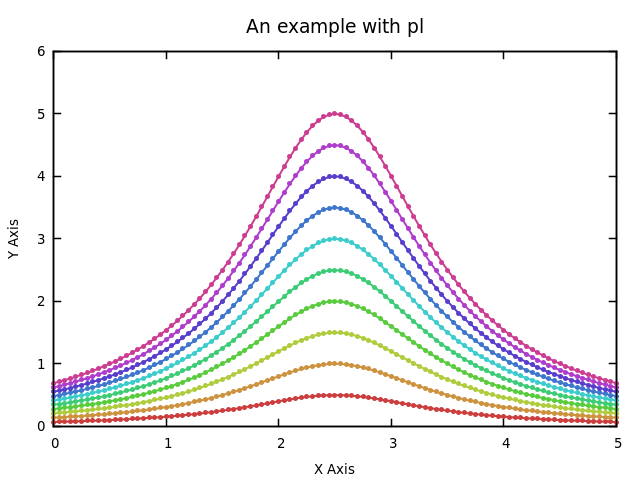
\includegraphics[width=\textwidth]{../../images/example.png}
    \vspace{0.3cm}
}

\author{\textbf{\autor}}                            % Autor
\date{\today}                                             % Fecha.
 
%----------------------------------------------------------------------------------------

\begin{document}

\maketitle

%----------------------------------------------------------------------------------------
%	ÍNDICE
%----------------------------------------------------------------------------------------

% Profundidad del Índice:
%\setcounter{tocdepth}{1}

\newpage
\tableofcontents
\listoflistings      % Lista con los códigos. Borrar si se desea.
\newpage

%----------------------------------------------------------------------------------------
%	Sección 1: Introducción
%----------------------------------------------------------------------------------------

\section{Introducción}

	Una tarea habitual de los informáticos es crear gráficas para comparar resultados de diferentes algoritmos. Los algoritmos surgen de forma natural en cualquier área de la informática. Por tanto, rara es la asignatura de la carrera en la que no se pida implementar varios de ellos y realizar un estudio comparativo. En este ámbito, las gráficas son esenciales para sintetizar la información obtenida durante las ejecuciones.

	Consecuentemente, hay que recurrir a programas para realizar estas gráficas. Aquellos similares a Excel son muy utilizados. En estos el proceso de creación de las gráficas es intuitivo y visual pero bastante lento. Cada vez que se obtienen nuevos datos hay que repetir el mismo procedimiento manual para generar la gráfica asociada. 
	
	Es más productivo un lenguaje de programación mediante el cual se programe cómo debe ser la gráfica. De esta forma se puede ejecutar el código automáticamente dentro de un script que trate los datos. Además, el código redactado es reutilizable. Varias opciones son:
	
	\begin{itemize}
		\item Lenguajes interpretados de propósito general, como Python, que suelen disponer de librerías extensas para la creación de gráficos. En el caso de Python cabe destacar \texttt{matplotlib} [1].
		\item El lenguaje de programación R, que está enfocado al análisis de datos [2]. R dispone de librerías con mucha funcionalidad para generar gráficos, como \texttt{ggplot2} [3].
		\item Gnuplot, que es un lenguaje específico para la creación de gráficos [4]. Gnuplot da mucha libertad al usuario para personalizar sus gráficas pero, como consecuencia, el aprendizaje es dificultoso. Es más, el código necesario para crear una gráfica puede tener fácilmente 50 líneas.
	\end{itemize} 
	
	En cualquier caso, hay que aprender un nuevo lenguaje de programación y trabajar con código para ello. Además, cada vez que se quiera añadir nuevos datos a la gráfica hay que modificar bastante el código correspondiente.
	
	El objetivo de esta práctica es proporcionar un comando para la terminal que permita crear gráficos de forma sencilla, intuitiva y automática y que utilice \textit{Lex} para tratar la entrada [5]. Para ello se genera un script con código de Gnuplot a partir de las opciones que ha indicado el usuario en la entrada.

%----------------------------------------------------------------------------------------
%	Sección 2: ¿Por qué usar Lex?
%----------------------------------------------------------------------------------------

\section{¿Por qué utilizar \textit{Lex}?}

	Se pretende que el comando sea lo más intuitivo posible. Por tanto, los argumentos o parámetros deben ser independientes de la posición en la que se escriban, como sucede en los comandos de bash. \textit{Lex} permite conseguir esto mediante la búsqueda de expresiones regulares en la entrada. Cada posible argumento se representa mediante una expresión regular a la que se le asocia la acción correspondiente. 
	
	Mediante este método el procesamiento de la entrada es lineal. Además, el código asociado se simplifica gracias a la sintaxis de \textit{Lex}. \textit{Lex} también permite comprobar que los datos dados como argumentos cumplan el léxico que se desea para ellos. Consecuentemente, evita muchas comprobaciones tediosas en el código. En la Sección \ref{sec:pl:arguments} se profundiza en las expresiones regulares utilizadas.
	
	\textit{Lex} habitualmente se utiliza para buscar en ficheros palabras aceptadas por expresiones regulares. Sin embargo, también se puede asignar como entrada una cadena de c mediante el comando \footnote{¿Cómo utilizar \texttt{yy\_scan\_string} en \textit{Lex}?: stackoverflow.com/questions/1907847/how-to-use-yy-scan-string-in-lex}:
	
	\mint[bgcolor=bg]{c}|void yy_scan_string(const char* str);|

	Por tanto, se puede utilizar \textit{Lex} para tratar los argumentos de un programa uniendo previamente estos en una nueva cadena. Este proceso es el que se realiza en \texttt{pl}. En esta práctica se propone el uso de \textit{Lex} como alternativa a un tratamiento de argumentos en C++ puro.

%----------------------------------------------------------------------------------------
%	Sección 3: ¿Cómo funciona pl?
%----------------------------------------------------------------------------------------

\section{¿Cómo funciona \texttt{pl}?}

	En esta sección se explica el funcionamiento del comando. En primer lugar se muestra qué puede hacer \texttt{pl} mediante un ejemplo. Posteriormente se profundiza en la sintaxis de \texttt{pl} explicando las expresiones regulares asociadas en \textit{Lex}.

	\subsection{¿Qué se puede hacer con \texttt{pl}?}

		Para usar \texttt{pl} solo hay que ejecutar el comando sobre un archivo con los datos. La Figura \ref{fig:example1} muestra la imagen obtenida por el Código \ref{listing:pl_example}.

        \begin{figure}[H]
        	\centering
			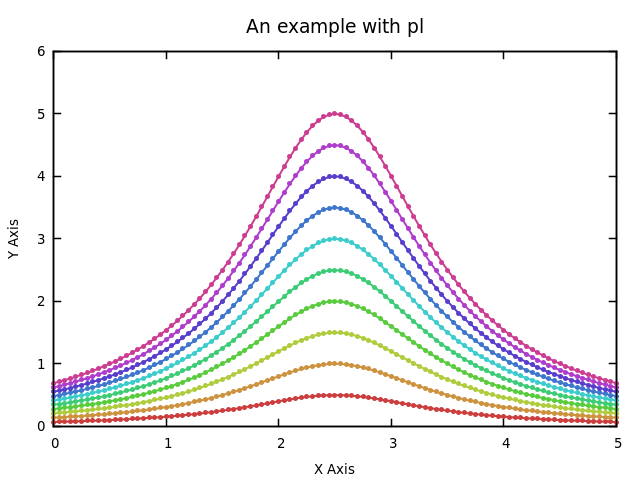
\includegraphics[width=0.8\textwidth]{../../images/example.png}
        	\caption{Una gráfica obtenida por \texttt{pl}.}
        	\label{fig:example1}
        \end{figure}

		\begin{listing}
			\caption{Ejemplo de uso de \texttt{pl}.}
			\begin{minted}[bgcolor=bg]{bash}
pl -e # Genera el archivo example.csv
pl example.csv -t "An example with pl" -x "X Axis" -y "Y Axis"
			\end{minted}
			\label{listing:pl_example}
		\end{listing}

		\texttt{pl} solo soporta gráficos en dos dimensiones en los cuales hay varios conjuntos de puntos distinguibles mediante colores. Estos son los gráficos más utilizados habitualmente en informática y el objetivo es que se puedan hacer lo más fácilmente posible.

		Para realizar los gráficos \texttt{pl} genera un archivo \texttt{plot.sh} que contiene las sentencias de Gnuplot necesarias y que se ejecuta mediante bash.
	
	\subsection{Archivos aceptados por \texttt{pl}} \label{sec:pl:arguments}
		
		\texttt{pl} puede utilizar múltiples archivos para una única gráfica. Los archivos aceptados por \texttt{pl} deben contener al menos dos columnas de números reales separadas por un delimitador. La primera columna se corresponde con las abscisas de los puntos a dibujar. Las siguientes columnas contienen una ordenada por cada abscisa, determinando un punto. Los puntos en una misma columna se dibujan con igual color. Por ejemplo, el archivo dado en el Código \ref{listing:lines1} representa 4 líneas horizontales. Se puede generar una gráfica a partir de este mediante el comando \texttt{pl lines1.csv}.

		\begin{listing}
			\caption{Ejemplo de un archivo aceptado por \texttt{pl}.}
			\begin{minted}[bgcolor=bg]{bash}
0,0,1,2,3
1,0,1,2,3
2,0,1,2,3
3,0,1,2,3
			\end{minted}
			\label{listing:lines1}
		\end{listing}
		
        \begin{figure}[H]
        	\centering
        	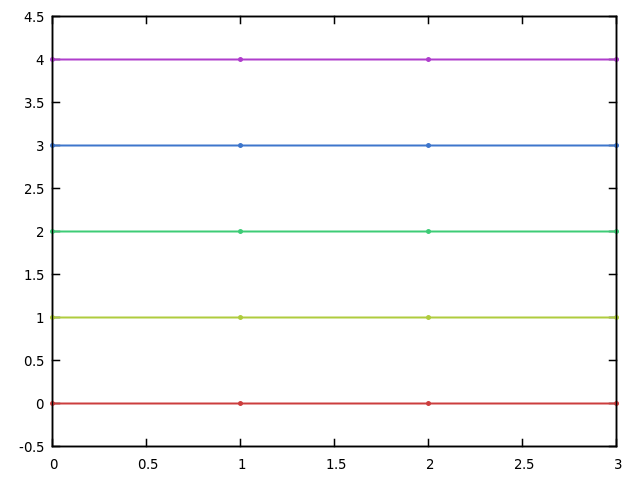
\includegraphics[width=0.6\textwidth]{../../images/lines1.png}
        	\caption{Gráfica asociada al fichero dado en el Código \ref{listing:lines1}.}
        	\label{fig:lines1}
        \end{figure}

		En el archivo del Código \ref{listing:lines1} se utiliza el estándar csv (una coma como separador). Sin embargo, se puede asignar un delimitador diferente mediante el argumento \texttt{-d <character>}. Este argumento responde a la siguiente expresión regular:
		
		\mint[bgcolor=bg]{bash}|-d{space}{char}|

		donde \texttt{space} es \texttt{[ \textbackslash t]*}	y \texttt{char} un carácter que puede estar delimitado o no por comillas.
 
		Normalmente los datos a utilizar están almacenados en diferentes ficheros y los puntos de los distintos conjuntos de datos no tienen necesariamente las mismas abscisas. \texttt{pl} puede utilizar varios ficheros para una misma gráfica, con la única restricción de que tengan el mismo delimitador. Por ejemplo, el comando \texttt{pl *.csv} haría una gráfica con los datos de todos los archivos csv del directorio. Si estos fuesen los archivos dados por los Códigos \ref{listing:lines1} y \ref{listing:lines2}, entonces el resultado es el mostrado por la Figura \ref{fig:lines1-lines2}.

		\begin{listing}
			\caption{Segundo ejemplo de un archivo aceptado por \texttt{pl}.}
			\begin{minted}[bgcolor=bg]{bash}
0,0.5,1.5,2.5,3.5
0.5,0.5,1.5,2.5,3.5
2.5,0.5,1.5,2.5,3.5
3,0.5,1.5,2.5,3.5
			\end{minted}
			\label{listing:lines2}
		\end{listing}

        \begin{figure}[H]
        	\centering
        	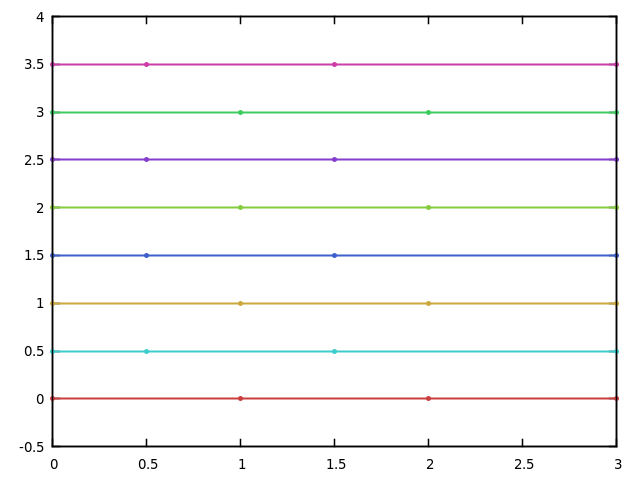
\includegraphics[width=0.6\textwidth]{../../images/both_lines.png}
        	\caption{Gráfica asociada los ficheros dados en los Códigos \ref{listing:lines1} y \ref{listing:lines2}.}
        	\label{fig:lines1-lines2}
        \end{figure}

		\texttt{pl} detecta los nombres de archivos como palabras sin espacios que contienen al menos un punto, a partir del cual todo se considera como extensión del archivo. Si un archivo no contiene ningún punto se debe utilizar el argumento \texttt{-f <file name>}, pudiendo introducir un número arbitrario de archivos entre comillas.

	\subsection{Argumentos de \texttt{pl}} \label{sec:pl:arguments}

		En esta sección se presentan los argumentos de \texttt{pl} que no se han mencionado previamente. Todos ellos siguen las expresiones regulares \texttt{-\{character\}}, \texttt{-\{character\}\{space\}\{word\}} o \texttt{-\{character\}\{space\}\{line\}}, donde una línea se considera como una sucesión de palabras y espacios delimitada por \texttt{"} o \texttt{'}.
	
		\begin{itemize}
			\item \texttt{-o\{space\}\{word\}} A la imagen creada se le asigna el nombre dado como argumento.

			\item \texttt{-t\{space\}(\{word\}|\{line\})} Asigna un título a la imagen. El título puede ser una palabra o una línea.
	
			\item \texttt{-x\{space\}(\{word\}|\{line\})} Asigna una etiqueta al eje de las abscisas. La etiqueta puede ser una palabra o una línea.
	
			\item \texttt{-y\{space\}(\{word\}|\{line\})} Asigna una etiqueta al eje de las ordenadas. La etiqueta puede ser una palabra o una línea.
				
			\item \texttt{-l} La primera entrada de cada columna de los ficheros se toma como leyenda del conjunto de puntos correspondiente. Además, si no hay etiqueta para el eje de las abscisas, entonces la primera entrada de la columna de las abscisas se utiliza como etiqueta.
		\end{itemize}

		Por ejemplo, el Código \ref{listing:lines_legend} muestra un archivo con leyenda. El siguiente comando aplicado sobre este archivo genera la Figura \ref{fig:legend}.
		
		\mint[bgcolor=bg]{c}|pl legend.csv -o my_plot.png -l -t "Some lines with legend." -y "Y Axis"|
	
		\begin{listing}
			\caption{Ejemplo de un archivo aceptado por \texttt{pl} con leyenda.}
			\begin{minted}[bgcolor=bg]{bash}
X Axis,Line 1, Line 2, Line 3, Line 4
0,0,1,2,3
1,0,1,2,3
2,0,1,2,3
3,0,1,2,3
			\end{minted}
			\label{listing:lines_legend}
		\end{listing}

       \begin{figure}[H]
	       	\centering
	       	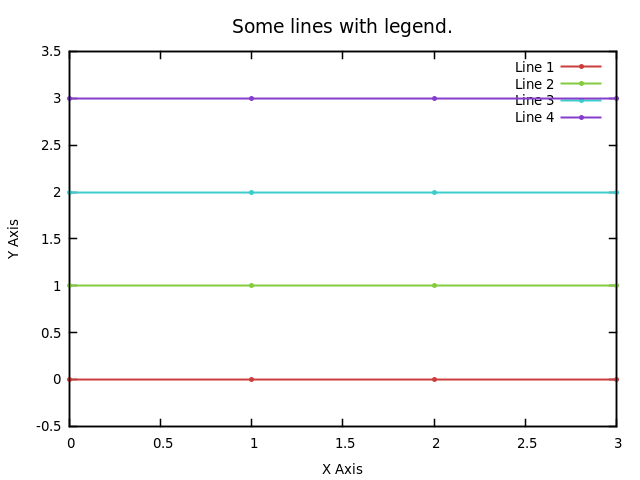
\includegraphics[width=0.6\textwidth]{../../images/my_plot.png}
	       	\caption{Gráfica con leyenda asociada al fichero dado en el Código \ref{listing:lines_legend}.}
	       	\label{fig:legend}
       \end{figure}

		Por defecto \texttt{pl} dibuja los conjuntos de puntos unidos por líneas. Sin embargo, también se pueden dibujar puntos o líneas solas.

		\begin{itemize}
			\item \texttt{-s\{space\}\{style\}} Cambia el estilo del gráfico. Hay tres estilos factibles: \texttt{lines}, \texttt{points} y \texttt{linespoints}. Cada uno de ellos tiene su correspondiente abreviación: \texttt{l}, \texttt{p} y \texttt{lp}.
			
			\item \texttt{-w\{space\}\{number\}} Cambia el ancho de línea por el número natural dado como parámetro. El ancho de línea es 2 por defecto.
		\end{itemize}
		
		Para ver la ayuda desde la terminal se puede utilizar el comando \texttt{pl -h}. Por otro lado, si se desea consultar el archivo \texttt{plot.sh} generado para crear la gráfica se puede utilizar el argumento \texttt{-k}, que evita que se elimine tras la ejecución.
		
	\subsection{Colores utilizados en las gráficas}
		
		Para seleccionar los colores de las gráficas \texttt{pl} utiliza el espacio HSV [6]. En este espacio los colores se representan por tres componentes:

		\begin{itemize}
			\item \textbf{Tonalidad}. Informalmente se entiende como la sensación visual según la cual el área coloreada se asemeja a uno de los tres colores básicos (rojo, verde y azul) o a una combinación de dos de ellos. Formalmente se corresponde con un ángulo (normalizado en [0,1)) que indica la posición del color en la circunferencia circunscrita al triángulo equilátero cuyos vértices son el rojo, el verde y el azul (en ese orden y comenzando el rojo en 0).

			\item \textbf{Brillo}. Se define como la cantidad de luz que refleja el color observado. Esto puede medirse como su distancia al color blanco normalizada.

			\item \textbf{Saturación} Se define como la intensidad del color divida por el brillo. También se normaliza en [0,1].
		\end{itemize}

		La transformación entre RGB y HSV es estándar y se puede encontrar con gran cantidad de detalles en la literatura. \footnote{Artículo extenso sobre los modelos de color HSV y HSL: https://en.wikipedia.org/wiki/HSL\_and\_HSV}

		Por defecto, \texttt{pl} toma colores con igual saturación y brillo. La tonalidad se elige uniformemente en el intervalo [0,1). Exactamente, se toman los valores $\frac{i-1}{n} \ \forall i = 1 \ldots n$, donde $n$ es el número de colores necesarios. De esta forma se garantiza que los colores sean distintos entre sí pero mantengan cierta concordancia.

		\texttt{pl} también permite elegir colores con similar tonalidad. Para ello toma como argumento el color elegido y varía el brillo uniformemente sin llegar a colores muy oscuros. La saturación varía un poco para garantizar ciertas diferencias entre los colores. Se proporcionan dos argumentos para esto:

		\begin{itemize}
			\item \texttt{-c\{space\}\{color\_name\}} : Los colores se eligen como variaciones del color dado como argumento. Se puede escoger entre rojo, amarillo, verde, azul, cian, y magenta.
		
			\item \texttt{-c\{space\}\{color\_rgb\}} : Los colores se eligen como variaciones del color dado como argumento. Este consiste en una tupla R,G,B con la representación RGB del color escogido. Cada valor es un entero entre 0 y 255.
		\end{itemize}		

		El primer argumento simplemente transforma el color escogido a RGB para realizar los cómputos. Por ejemplo, la Figura \ref{fig:color} muestra una gráfica realizada con cian.

		\begin{figure}[H]
	       	\centering
	       	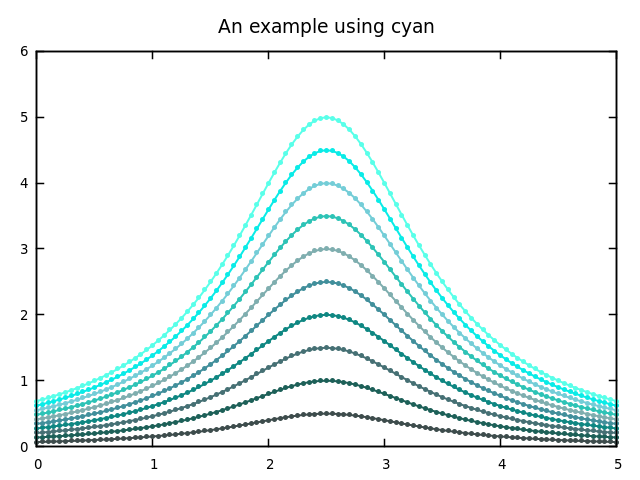
\includegraphics[width=0.8\textwidth]{../../images/example_cyan.png}
	       	\caption{Gráfica donde se ha utilizado el argumento \texttt{-c cyan}.}
	       	\label{fig:color}
		\end{figure}

%----------------------------------------------------------------------------------------
%	Sección 4: Conclusión
%----------------------------------------------------------------------------------------

	\section{Conclusión}

		El uso de \textit{Lex} para tratar los argumentos de un programa facilita al programador esta sección del código. Las expresiones regulares proporcionan un mecanismo de detección de parámetros sencillo y eficaz, controlando además el léxico de los parámetros leídos.
	
		Este hecho se prueba mediante la redacción de un programa para la creación de gráficas dos dimensionales, que se propone como una alternativa sencilla e intuitiva frente a las librerías utilizadas para este propósito. El programa presenta una completa selección de argumentos y automatiza todos los procesos asociados a la creación de gráficas. Además, los colores utilizados por este se eligen de forma que sean diferentes entre sí pero mantengan cierta concordancia.
	
		\textit{Nota: El código se encuentra alojado en https://github.com/andreshp/pl}
	
%----------------------------------------------------------------------------------------
%	Sección 5: Bibliografía
%----------------------------------------------------------------------------------------

\section{Bibliografía}

	\begin{enumerate}
		\item Hunter, John D. ``Matplotlib: A 2D graphics environment.'' Computing in science and engineering. Año 2007. Páginas 90-95.
		\item Team R Core. "R Language Definition.'' Año 2000.
		\item Wickham, Hadley. ``ggplot2: elegant graphics for data analysis." Springer Science and Business Media. Año 2009.
		\item Janert, Philipp K. ``Gnuplot in action.'' Manning. Año 2010.
		\item Lesk, Michael E., y Eric Schmidt. ``Lex: A lexical analyzer generator.'' Año 1975.
		\item Tkalcic, Marko, y Jurij F. Tasic.``Colour spaces: perceptual, historical and applicational background.'' Eurocon. Año 2003. Páginas 304-308.
	\end{enumerate}

\end{document}